\chapter{Manual}

\subsubsection{Indexador}

Para realizar la indexación hay que ejecutar el programa
\texttt{index.py} con los parámetros que exigen los requisitos de la
práctica, se adjunta un ejemplo de como se debería de lanzar:

\begin{lstlisting}
./indexer.py iniciativas08 palabras_vacias_utf8.txt index
\end{lstlisting}

\begin{quote}
Si no se le especifican los parámetros requeridos el programa mostrará
un mensaje de ayuda.
\end{quote}

\begin{figure}
\centering
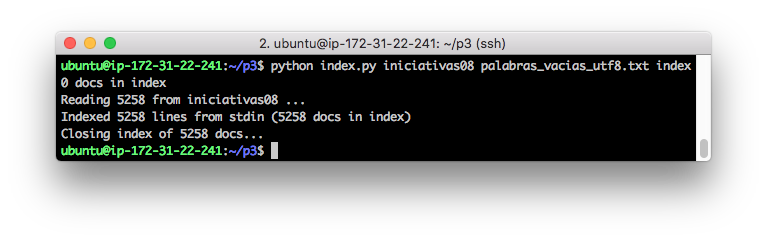
\includegraphics[width=1.0\textwidth]{../images/index.png}
\caption{Indexador}
\end{figure}

\subsubsection{Motor de Búsqueda}

Para lanzar el motor de búsqueda hay que ejecutar el programa
\texttt{search.py} con los parámetros que exigen los requisitos de la
práctica, se adjunta un ejemplo de como se debería de lanzar:

\begin{lstlisting}
./search.py index
\end{lstlisting}

\begin{quote}
Si no se le especifican los parámetros requeridos el programa mostrará
un mensaje de ayuda.
\end{quote}

\begin{figure}
\centering
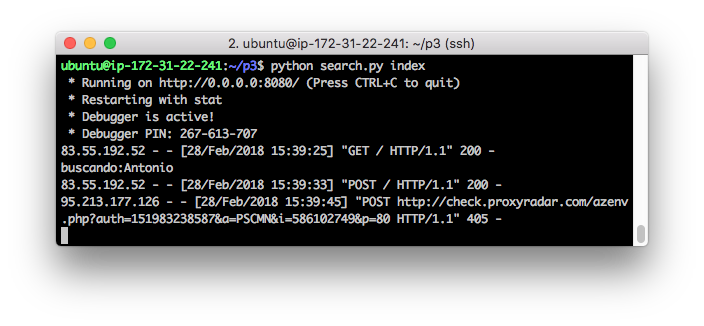
\includegraphics[width=1.0\textwidth]{../images/search.png}
\caption{Motor de búsqueda}
\end{figure}

Una vez lanzado el programa podremos interactuar con el buscador
entrando con el navegador en la url \url{http://localhost:8080}